\section{Teoría de Acoplamiento}
\label{coupling_theory}

En la figura \ref{fig:rr_model} se muestra el esquema del caso genérico de un anillo resonador con 2 regiones de acoplamiento representadas por las líneas punteadas. 
Dentro de los parámetros del sistema se encuentran  
$\kappa_{1},\kappa_{1}^{*}\kappa_{2}\kappa_{2}^{*}$ que representan los coeficientes de acoplo 
y $t_{1}, t_{*}, t_{2}, t_{2}^{*}$ que representan los coeficientes de transmisión.

\begin{figure}[h!]
\caption{Modelo de un Anillo Resonador}
\centering
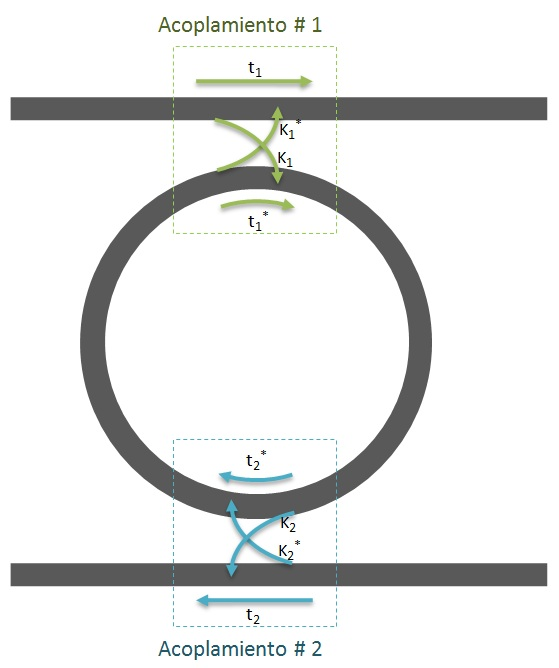
\includegraphics[width=0.5\textwidth,natwidth=559,natheight=668]{figs/rr_model.jpg}
\label{fig:rr_model}
\end{figure} 

%TODO explicar q estamos hablando de As%
La potencia de la onda que se ve en el puerto 2 está dada por la porción de la onda incidente
que atravieza la guía más las $N\to\infty$ contribuciones que se dan por la otra parte de la
onda que se acopló en el anillo (ec. \ref{eq:coupling_gral}).

\begin{equation}
A_s = A_i t_1 + Contrib_{N=1} + Contrib_{N=2} + ... + Contrib_{N=\infty}
\label{eq:coupling_gral}
\end{equation} 

Cada una de las contribuciones depende del número de viajes completos que realice la onda
acoplada antes de volver a salir a la guía superior.
Se explicarán las 2 primeras contribuciones y de allí se procederá a 
generalizar y resolver la ecuación:

\begin{figure}[h!]
\caption{Contribución Onda 1 Vuelta}
\centering
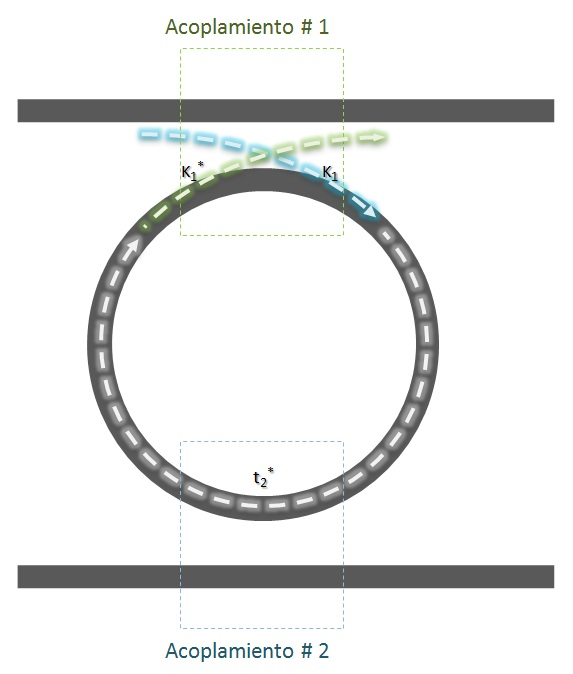
\includegraphics[width=0.5\textwidth,natwidth=573,natheight=674]{figs/rr_n1.jpg}
\label{fig:rr_n1}
\end{figure} 

En la figura \ref{fig:rr_n1} se muestra el viaje que realiza
la onda acoplada al dar una sola vuelta y salir. 
Como se aprecia, la onda inicial $A_i$ que no continúa su trayectoria recta es acoplada dentro 
del anillo por un factor $\kappa_1$. 
La transmisión alrededor del anillo está atenuada por $e^{-j \beta L}$.
Una vez la onda llega al acoplamiento No 2 (guía inferior), sólo una porción
dada por el factor $t_2^*$ sigue su recorrido dentro del anillo. 
Finalmente, la onda completa una vuelta y se acopla, por un factor $\kappa_1^*$, 
a la guía original (ec .\ref{eq:coupling_round_1}).

\begin{equation}
Contrib_{N=1} = A_i \kappa_1 \kappa_1^* t_2^* e^{-j \beta L}
\label{eq:coupling_round_1}
\end{equation} 

Sin embargo, existe una porción de esta onda que no vuelve a la guía 1, sino que atravieza 
la región de acoplamiento No 1 por un factor $t_1^*$ (ver Figura \ref{fig:rr_n2}. Nuevamente pasa por la región
de acoplamiento No 2 y sigue su trayectoria dentro del anillo multiplicada por otro factor
$t_2^*$ y por otra atenuación $e^{-j \beta L}$. 
Finalmente, completa 2 vueltas y se acopla por un factor $\kappa_1^*$ a la guía 
original (ec. \ref{eq:coupling_round_2}).

\begin{figure}[h!]
\caption{Contribución Onda 2 Vueltas}
\centering
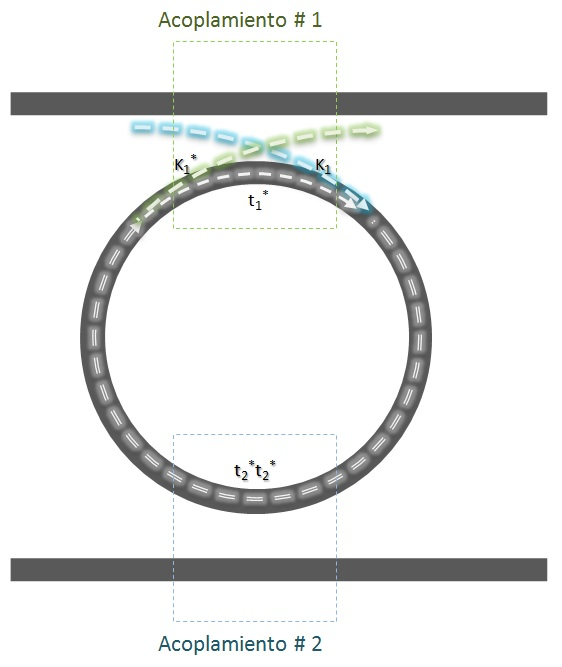
\includegraphics[width=0.5\textwidth,natwidth=562,natheight=667]{figs/rr_n2.jpg}
\label{fig:rr_n2}
\end{figure} 

\begin{equation}
Contrib_{N=2} = A_i \kappa_1 \kappa_1^* t_2^* e^{-j \beta L} t_1^* t_2^* e^{-j \beta L}
\label{eq:coupling_round_2}
\end{equation} 

Y así, cada vez que la onda que completa otra vuelta completa llega al acoplamiento No 1,
existe una porción que no se acopla y da una vuelta más. Esta vuelta adicional incluye 
volver a atravezar los acoplamientos No 1 y 2 más el término de atenuación $e^{-j \beta L}$.
Por lo tanto, generalizando, se llega a la ecuación \ref{eq:coupling_sum} \cite{yariv2006photonics}.

\begin{equation}
A_s = A_i\{
t_1+
\kappa_{1} \kappa_{1}^{*} t_{2}^{*} e^{-j \beta L} (
1 +
t_{1}^{*} t_{2}^{*} e^{-j \beta L} +
(t_{1}^{*} t_{2}^{*} e^{-j \beta L})^{2} +
...)\}
\label{eq:coupling_sum}
\end{equation}


Al analizar estas contribuciones cuando $N \to \infty$ se llega a la ecuación 
\ref{eq:coupling_sum}. Al ser una serie geométrica infinita, su solución está dada por la
ecuación \ref{eq:geom_series}:

\begin{equation}
\sum\limits_{k = 0}^\infty {ar^{k} = \frac{a}{{1 - r}}}  
\label{eq:geom_series}
\end{equation} 

Donde, 

\begin{align}
a &= \kappa_{1} \kappa_{1}^{*} t_{2}^{*} e^{-j \beta L} \\ 
r &= t_{1}^{*} t_{2}^{*} e^{-j \beta L}
\end{align} 

Por lo tanto:
\begin{equation}
A_s = A_i\{t_1 + 
\frac{ \kappa_{1} \kappa_{1}^{*} t_{2}^{*} e^{-j \beta L}}
{1 - t_{1}^{*} t_{2}^{*} e^{-j \beta L}} \}
\end{equation} 
